\documentclass[]{article}
\usepackage{graphicx}
\usepackage{hyperref}
\usepackage{siunitx}

\usepackage{framed}

\input{/home/lorilan/thesis/common_macros.tex}
\input{/home/lorilan/thesis/java_listing.tex}




%opening
\title{Puck manual}
\author{}

\begin{document}

\maketitle

\begin{abstract}

\end{abstract}

\section{User Interface}

Puck's interface is composed of four panels(cf figure \ref{fig:screenshot}). 

\begin{figure}
	\centerline{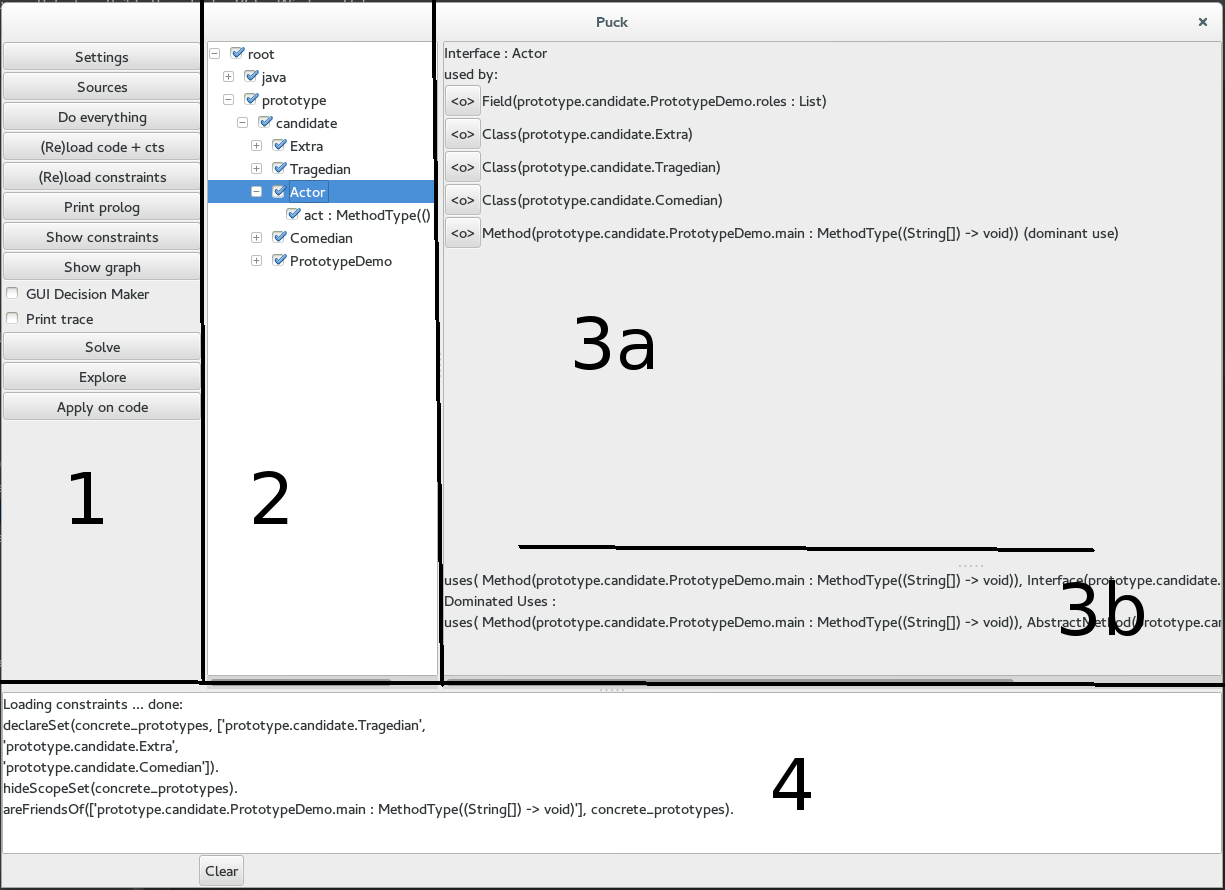
\includegraphics[keepaspectratio, width=1.7\textwidth]{screenshot.png}}
	\caption{Screen-shot of main panel of puck}
	\label{fig:screenshot}
\end{figure}

\begin{enumerate}
\item the button panel
\item the package explorer
\item the node information panel
\item the console
\end{enumerate}

Settings and global control is done in the button panel. Once an access graph is loaded, you can browse the different nodes in the package explorer. When you click on a node, detailed information are displayed on the node information panel. The console displays various informations. You can clear it at any time with the \verb|Clear| button. The button panel and the node information panel are detailed below.

\subsection{Button Panel}
\subsubsection{Simple use}

A normal work space for puck is composed by a folder containing java sources (1.4 or 1.5).
A file named \verb|decouple.pl| placed at the root of the work space.

Optionally the following input can also be given to puck by placing them at the root of the work space :
\begin{itemize}
\item \verb|jar.list| : A file containing a list of absolute paths to jar archives (one per line), if the sources requires external libraries to compile.
\item \verb|api_nodes| : A list of elements of the java standard library that you wish to see displayed on the graph.
\end{itemize} 

The most simple use case, if you have a work space containing the above mention files with the default name and path, you just have to select it with the
 \verb|Work space| button and press \verb|Dot it !|\footnote{puck takes the directory from where it was open as its default work space, so if you open puck from your work space root you just have to click Dot it !}.
 Puck will then 
 \begin{enumerate}
 	\item load the Java sources and create an access graph
 	\item load the coupling constraints
 	\item display the access graph with violations marked in red
 	\item solve the constraints with a default strategy
 	\item display the solved access graph
 	\item apply the computed change on the source code
 	\item open the original sources and the modified ones 	
 \end{enumerate}

\subsubsection{Buttons decsription}

\begin{itemize}
	\item \verb|Settings|\\
	Open a window when you can change the default values.\\
	\important{Puck relies on Graphviz dot\cite{graphviz} to generate the visual version of the graph. If it is not accessible from your PATH system variable, you need to set dot executable path in this setting window.}
	
	\item \verb|Work space|\\
	Let you choose a work space and try to load the source code.
	
	\item \verb|Do it !|\\
	Do the process described above.
	
	\item \verb|(Re)load code & constraints|\\
	(Re)load the code from the current source path. If you edit your sources outside of puck, or if you open puck at the root directory of your sources files you can (re)load them with this button. It will also load the constraint file.
	
	\item \verb|(Re)load constraints|\\
	This will remove any loaded constraint on the graph and reload the constraint file. Useful while you are editing your constraint file.
	
	\item \verb|Print prolog|\\
	This print a prolog representation of the access graph.
	
	\item \verb|Show constraints|\\
	Print the loaded constraint in the console.
	
	\item \verb|Show graph|\\
	Display a graphic version of the access graph with constraint violations in red.
	
	\item \verb|GUI Decision Maker|\\
	Check this box to take the decision instead of the default strategy during the solving process.\\
	\todo{Finish implementation}
	
	\item \verb|Print trace|\\
	Check this box to create png files of the graph at each iteration of the solving process (work also for ``exploration'').
	
	\item \verb|Solve|\\
	Launch the solving process.
	
	\item \verb|Explore|\\
	Explore all choices during the solving process. Create png files of all the results. At the end of the process the graph state is the last one explored.
	\todo{Implement a menu to navigate between the solutions}
	
	\item \verb|Apply on code|\\
	Apply the changes computed to obtain the current code on the underlying representation of the code a reprint it in the output directory.
	
\end{itemize}

\subsection{Node information panel}
This screen is divided in two parts (cf 3a \& 3b on figure \ref{fig:screenshot}).
When you select a node in the package explorer, on the top of the node information panel, you can see the users of the selected node. If you click on the \verb|<o>| button next a user, it will display the graph with the uses (user, selected node) in bold, its dominant uses (if any) in blue and its dominated uses (if any) in green.
This information can also be accessed textually. The list of the dominant and dominated uses can be displayed at the bottom of the panel by clicking on the user node name.

\section{Constraint}
The parsed constraints have the following formal grammar:\footnote{facades, interlopers and friends are always scope sets}

\begin{itemize}
	\item $constraintFile$ \verb|::=(|$clause$\verb|)*| 
	
	\item \begin{tabbing}
		$clause$ \verb|::|\=\verb|=| java\_import($list$).\\		
		\>$|$ declareSet($ident$, $list$).\\
		\>$|$ declareSetUnion($ident$, $list$).\\
		\>$|\; constraint$
	\end{tabbing}
	\item \begin{tabbing}
		$constraint$ \verb|::|\=\verb|=| hideScope($ident$, $listOrIdent$, $listOrIdent$, $listOrIdent$).\\	
		\>\color{light-gray}{hideScope(scope, facades, interlopers, friends)}\\
		
		\>$|$ hideScopeSet($listOrIdent$, $listOrIdent$, $listOrIdent$, $listOrIdent$).\\
		\>\color{light-gray}{hideScopeSet(scopeSet, facades, interlopers, friends)}\\
		
		\>$|$ hideScopeSet($listOrIdent$).\\
		\>\color{light-gray}{hideScopeSet(scopeSet)}\\
			
		\>$|$ hideScopeSetFrom($listOrIdent$, $listOrIdent$).\\
		\>\color{light-gray}{hideScopeSetFrom(scopeSet, interlopers)}\\
			
		\>$|$ hideScopeFromEachOther($listOrIdent$).\\
		\>\color{light-gray}{hideScopeFromEachOther(scopeSet)}\\
		\\
		\>$|$ hide($ident$, $listOrIdent$, $listOrIdent$).\\
		\>\color{light-gray}{hide(element, interlopers, friends)}\\
		
		\>$|$ hideSet($listOrIdent$, $listOrIdent$, $listOrIdent$).\\	
		\>\color{light-gray}{hideSet(elementSet, interlopers, friends)}\\
		
		\>$|$ hideFrom($ident$, $listOrIdent$).\\	
		\>\color{light-gray}{hideFrom(element, interlopers)}\\
				
		\>$|$ hideSetFrom($listOrIdent$, $listOrIdent$).\\	
		\>\color{light-gray}{hideSetFrom(elementSet, interlopers)}\\
		\\
		
		\>$|$ isFriendOf($listOrIdent$, $listOrIdent$).\\
		\>\color{light-gray}{isFriendOf(scopeSet, beFriended)}\\
		
	\end{tabbing}

	\item \begin{tabbing}
		$ident$ \verb|::|\=\verb|=[^|[]',().\verb|]+|\\		
		\>$|$ '\verb|[^|'\verb|]+|'
	\end{tabbing}
	
	\item $list$ \verb|::=| [ ] $|$ [$ident$\verb|(|,$ident$\verb|)*|]\\		
	
	\item $listOrIdent$ \verb|::=| $list\; |\; ident$\\		
		
\end{itemize}


\section{Puck's Architecture}
Puck is written in scala. 
It is build in top of JastAddJ \cite{ekman2007jastaddj} and Jrrt \cite{jrrt, schafer2012accessibility}.
\subsection{Legacy code}
AST of JastAddJ\\
Some functions introduced by Jrrt (uses() ! + lexer/parser rewritten using beaver)\\
AST generate Access Graph (Composed of generic parts + java/JasAddJ specific binders)


\subsection{New parts}
Its architecture is composed of the following packages: 
\begin{itemize}
\item \verb|puck|\\
	It is the root package, it contains only the Front object

\item \verb|puck.graph|\\
	This package and its subpackages contains the generic elements of the access graph. A lot of classes including AccessGraph and AGNode are parameterized by the node kind. This package contains mainly the classes describing the structure of the graph and its node.

\item \verb|puck.graph.backTrack|\\
	Even if scala promotes the functional paradigm, the main purpose of puck is to compute modification on potential huge access graph. For this reason, AccessGraph and AGNode are mutable structure. This package contains what is necessary to undo/redo modification applied on the access graph.

\item \verb|puck.graph.constraints|\\
	It is here that we find the classes that relate to the constraints. It goes from the parser to the solver.

\item \verb|puck.graph.io|\\
	To graph printer are here. We also find here the FilesHandler : this class give some high level interface about the graph processing.

\item \verb|puck.gui|\\
	This package gather together the puck's graphical interface. As in \verb|puck.graph| the classes found here are generic and deals with generic AccessGraph.
	
\item \verb|puck.gui.decisionsFrames|\\
	This sub-package contains the different panel that let the user make its decisions when the constraint solving process offers several possibility.
	
\item \verb|puck.javaAG|\\
	All java specific material is gathered here. 
	In particular we find the AG2AST object that apply on the AST the transformations computed on the access graph.

\item \verb|puck.javaAG.nodeKind|\\
	This package contains the java node kind. Some language specific consideration about graph transformations are black boxed here.

\item \verb|puck.search|\\
	Contains a generic search engine framework. It is used both in the constraint solving process and in the graph transformation recording comparator.

\item \verb|puck.util|\\
This package contains 
\begin{itemize}
\item a generic breadth first iterator for trees
\item a mini logger framework
\item some basic file helper functions and a timer
\end{itemize}
\end{itemize}


\paragraph{puck.search} The search engine is coded and meant to be used in a continuation passing style

\section{Solver built-in strategy}
The solver trait (\verb|puck.graph.constraints.Solver|) uses a decision maker. A decision maker is an interface that abstract how decision are made. Three implementations can be found in puck:
\begin{itemize}
	\item \verb|puck.graph.constraints.DefaultDecisionMaker|\\
	This decision maker make decisions based on a heuristic that will be explained in section \ref{section:defaultDecisionMaker}.
	\item \verb|puck.gui.GUIDecisionMaker|\\
	This implementation uses windows to ask the user which decision to make. \todo{Implementation to finish}
	\item \verb|puck.graph.constraints.ConstraintSolvingSearchEngine|
	This implementation is based on the search engine. At a decision point it compute all the possible solutions. All choices can be explored thanks to backtrack.
\end{itemize}

However some decisions are hard coded. Some are imposed by the fact that the solving process is done on an access graph and we rely on the available information.
Other are the product of a heuristic to reduce the search state space. This choices are what is called the built-in strategy and explained here:

\subsection{Main loop}
The main loop of the solver searches for violations target, then tries to solve as many of the violations with the same target as possible. Then it loops and do it again until there is no more violation.\\

The decision of the violation target is delegated to the decision maker.

Two kinds of arcs can be labeled as violations : \textuses{} and \textcontains.

To remove a contains violation, we move the target into another host.

To remove a \textuses{} violation we redirect it toward an abstraction of the target, in general a super type. Redirecting the source of a \textuses{} arc in term of code means doing an extract method. This refactoring is not computable on the access graph since to do it properly we need precise information about the context in which an element is used. The access graph does not give such informations.

For a given violations target $t$, if the \textcontains{} arc (\_, $t$) is a violation, we solve it before the \textuses{} violations.
If we solve the uses violations first, however $t$ is abstracted it won't change $t$ container and this contains violation will still have to be solved.
While when choosing a new host for $t$, we can find a host such that is also solves uses violations, thus preventing the creation of an uneeded abstraction that would complicate the software architecture.

\subsection{Removing contains violation}
As said above, to remove a contains violation, we move the target into another host. If there is no suited host, a new one is created.
The choice of the host is delegated to the decision maker.
In case of an unsolvable coupling problem, caused by a constraint hiding an element from anything, a new host is created and an exception is automatically added:
\verb|hide('A')| is transformed into \verb|hideButFrom('A', ['A_container'])|

\cmt{Ajouter exception pour les uses quand toute les violations ont pour origine le même noeud ?\\
Ou mettre une exception "globale" pour le main}

\subsection{Removing uses violation}
We create a new abstraction after having failed to find an existing one. The decision of the kind and the policy of the abstraction is delegated to the decision maker. With the information of the access graph, we can assume that if A is a B (there is an ``isa'' arc between A and B) then B is a potential abstraction for A. Outside of that we have to rely on the abstraction mapping produced while creating the graph (how to build is thus a language dependent issue).

The policy of the abstraction is \emph{super type} or \emph{delegate}. In the most general fashion, the difference between the two policies is that with \emph{super type}, the abstracted node uses its abstraction while with \emph{delegation} it's the abstraction that uses the abstracted node.

By which node kind another kind can be abstracted depends of the abstraction's policy. Both policy are not always available.

For instance in java neither a constructor nor a field can be abstracted using a super type strategy. In scala a field can be abstracted using super type.
In java an interface can be abstracted by super type policy only with another interface while if we use delegate policy it can only be abstracted by a class.
So which kind of strategy and abstraction kind is available for each kind is a language specific knowledge. 

 
Once these decisions are made, we ask the graph to build an abstraction, another language specific process. What is general is that this abstraction will need a host if we do not find one we will build one by abstracting the host of the node we were originally abstracting. This host will itself need a container and thus it can recursively create another host and so on.
The reason why the host is creating by using the abstraction process and not ``ex nihilo'' as for the contains violation removal process is to generalize the specific case of a method abstraction.
If we abstract a method using super type strategy, its potential host have to satisfy some restriction. It has to be an interface implemented by the class containing the abstracted method. This restriction will be automatically respected because of the abstraction building process.


After an abstraction is found or created, the next step is to redirect uses. The general algorithm is to redirect also the dependant uses but there some special cases that have to be handled in a language specific way.


\subsection{Hard coded choices}
\begin{itemize}
	\item for a given violations target, we solve the contain violation before the uses
	\item we try to find an acceptable host before creating a new one 
	\item the uses violations are solved by abstracting the target
	\item we try to find and use existing abstraction before creating a new one\\
		this prevents the proliferation of abstractions that would uselessly complicate the software design
	
	\item when searching a host, it has to satisfy a certain predicate\\
		$potentialHost\neq toBeContained\\
		 \wedge\; potentialHost.kind\; canContain\; toBeContained.kind\\
		 \wedge\; potentialHost.isMutable$
		\begin{itemize}
			\item for a moving node\\
			$\wedge\; \neg (potentialHost\; interloperOf\; toBeContained)$
			\item for the newly created host of a moving node\\
			$\wedge\; true$
			\item for a newly created abstraction
			\begin{tabbing}
			if \=super type abstraction\\
			\>$\wedge\; \neg(abstractedNode\; interloperOf\; potentialHost)$\\
			else if delegation abstraction\\
			\>$\wedge\; \neg(potentialHost\; interloperOf\; abstractedNode)$
			\end{tabbing}
			\item for an abstraction recursively created to host another abstraction
			$\wedge\; true$
		\end{itemize}
\end{itemize}

\paragraph{Java specifics}
We do not consider the static elements.


\section{DefaultDecisionMaker : explanation of the heuristic}
\label{section:defaultDecisionMaker}

A decision maker has the responsibility to decide
\begin{itemize}
\item which node targeted by violations will be handled by the solver
\item what abstraction policy and node kind will be used to abstract a node
\item which host to use when searching one
\end{itemize}

For the first two questions I paste here the subsection ``Decisions and heuristics'' of the documents couplingProblems/searchProblem.tex in my ``document'' git repository:


\begin{framed}

The decisions concern the arguments of the rules and the choice made on the existential quantifiers. They can be summarize as follows :
\begin{enumerate}
%\item \label{enum:rule_choice} which rule use ?
\item \label{enum:violation_target_choice} which node will a rule be applied on ?
\item \label{enum:strategy_choice} which kind of abstraction and strategy use ?
\item \label{enum:host_choice} which node choose as host when moving a node or creating an abstraction ?
\end{enumerate}

After solving manually constraints violations on code examples, a strategy emerged. This strategy guides the exploration of the search state. About question \ref{enum:violation_target_choice}, it seems reasonable when applying a rule on node to try to remove as many violations as possible. In java we solve violations targeting classes before the ones targeting methods. Abstracting a class with an interface and redirecting the methods' uses toward their abstraction in the interface can solve several violations in one step. 
In a more general way we establish a node kind priority list.
[...]\\
\emph{``Program to an interface, not an implementation''} (\cite{gamma1993gof} p.18) is a well known practice. It decouples software pieces and allow a better re-usability. In our problem, it means using super types rather than delegates. Thus to answer question \ref{enum:strategy_choice} we always favor the one other the second when possible (for example constructors cannot be used via polymorphism). \\
This make us go back to question \ref{enum:violation_target_choice}: we solve violation toward fields and constructor before solving violation toward classes. Then when solving violations toward classes, we will be to able include field and constructor abstractions signature in the interfaces abstracting the classes.
\end{framed}

About the host, since it has to respect the predicate given in argument, the choice is pretty limited. Actually we take the first node making the predicate true. Which node will be find first depends of the underlying iterator : we use a breadth first search through the access graph tree composed by the contains arcs.

\section{ConstraintSolvingSearchEngine : Exploring the search space}

Similar solutions

Obvious (for a human) wrong choices : prototype where prototype are dispatched in several packages 

Definitions of \cite{abdeen2009automatic} adapted to our AG definitions :
A dependency is a use

let $G$ be an access graph and $n$ a node of $G$.
The set of dependencies of $n$ is defined as:\\
$n_D \equalByDef n_{Ext.D}\cup n_{Int.D}$\\
\cmt{union of external and internal dependencies}\\
$n_{Ext.D} \equalByDef n_{Out.D}\cup n_{Inc.D}$\\
\cmt{union of outgoing and incoming dependencies}\\
$n_{Out.D} \equalByDef \{(uses, s, t)\in G \suchthat \containedByTrC{s}{n} \wedge \neg (\containedByTrC{t}{n}) \}$\\
$n_{Inc.D} \equalByDef \{(uses, s, t)\in G \suchthat \neg(\containedByTrC{s}{n}) \wedge \containedByTrC{t}{n} \}$\\
$n_{Int.D} \equalByDef \{(uses, s, t)\in G \suchthat \containedByTrC{s}{n} \wedge \containedByTrC{t}{n} \}$\\

\noindent$provides(G, p, c)\equalByDef \exists (uses, s, t) \in G \suchthat \containedByTrC{s}{c} \wedge \containedByTrC{t}{p} \wedge \neg((uses, s, t)\in c_{Int.D} )$\\
$providers(n) \equalByDef \{ p \in G  \suchthat p\neq n 
\wedge n.kind=p.kind 
\wedge provides(G, p, n) \}$\\
$clients(n) \equalByDef \{ c \in G  \suchthat c\neq n 
\wedge n.kind=c.kind 
\wedge provides(G, n, c) \}$

\noindent$CohesionQ(n) \equalByDef \frac{|n_{Int.D}|}{|n_D|}$\\
$CouplingQ(n) \equalByDef 1 - \frac{|providers(n) \cup clients(n)|}{|n_D|}$


\subsection{Recording comparison : another search problem}
When different path converge to the same graph we want to stop following the new path. Hence we do graph comparison or more precisely we compare the list of transformations done on the graph and try to find a mapping between the newly introduced node in both path.

prototype/actors\\
1944 results in \SI{2}{\second}  \SI{382192}{\micro \second}\\
comparison reduces to 54 different results (without merging)\\
comparison without sorting by coupling first :
\SI{57}{\second} \SI{495923}{\micro\second}\\
comparison with coupling sort first :
\SI{11}{\second} \SI{177939}{\micro\second}

around 54000 result in around 50s

filter 216 results in one hour Oo


\section{Preservation of welltypedness}

In order to preserve the behavior we preserve the welltypedness of the program. To remove coupling constraint violation, we introduce abstraction.
To abstract a class we create an interface and we redirect \textuses of the class on the interface. We use the super type wherever it is possible.

"normal" algorithm :\\
1) intro abstraction\\
2) foreach wrong user uses abstraction instead\\

when introducing a super type:\\
1) intro abstraction\\
2) foreach wrong user uses abstraction instead\\
3) bring back well typedness


\begin{figure}
\centerline{
\begin{minipage}[t]{.6\textwidth}
\lstinputlisting[language=prolog]{examples/extractSuperType/decouple.pl}\lstinputlisting{examples/extractSuperType/D.java}
\end{minipage}
\hfil
\begin{minipage}[t]{.6\textwidth}
\lstinputlisting{examples/extractSuperType/out/p/A_SuperTypeAbstraction.java}
\lstinputlisting[numbers=left,    
  numbersep=5pt,                  
  numberstyle=\tiny\color{light-gray},]{examples/extractSuperType/out/p/D.java}
\end{minipage}}
\caption{A code, its constraint and a wrong production}
\label{fig:wrongExtract}
\end{figure}

Figure \ref{fig:wrongExtract} describe a class D using a forbidden class A. C and DUser use A legitimately. When we redirect all wrong uses from \texttt{A} to \texttt{A\_SuperTypeAbstraction} and only them, we obtain the code on the right column.
This code is not well typed : 

\begin{itemize}
\item C.m requires an argument typed A hence line 19 is wrong since a is typed with \texttt{A\_SuperTypeAbstraction}.
\item D.m3 return a value typed \texttt{A\_SuperTypeAbstraction} hence allocation of line 35 is also wrong. 
\end{itemize}


\section{Merge}

When do we do the merge ?\\
hypothesis : no merge necessary on the candidate code

the merge can be done either after or during the constraint solving.
if we do it during the constraint solving, we can ask the operation only on nodes that are newly created wheres if we do it in the end we have to search over all nodes (or we can store which nodes are created)


For now the merge is done after the coupling constraint problem solving. It is completely language dependent.

In only merge identical interfaces given that redirecting the uses do not create new violations.

Cannot reason on the control flow \todo{but same uses target set can be looked in details ??}

What about merging methods ?  we can find heuristic based on names (see bridge example where printText and printGraphic should be merge in the interface as a unique print signature -> but then we have to divide the implementation in two classes)


\section{Graph comparison}
Solving constraint using a search engine generates many solutions (\textasciitilde 1700 for a code composed of 4 classes one interface and 2 methods per class). Among these solutions many are the same. They are considered different because we got them following a different path.
We need to automatically compare these graphs and only keep the different solution.

Instead of comparing directly the graphs, we compare the transformations we operated on them. Two sets of transformations $S_1$ and $S_2$ are considered equal if there exists a mapping between the newly introduced nodes such that $|S_1| = |S_2| \wedge \forall t_1 \in S_1, \exists t_2 \in S_2 \suchthat t_1 = t_2$

Why not comparing directly the graph ? 
\begin{itemize}
\item the starting graph is potentially really big : we want to compare only the newly introduced elements
\item the recording necessary for backtracking purposes already stores which elements are newly introduced so we uses them
\end{itemize}

\subsection{Normalizing the record}
First we need to normalize the record. The merging process introduces the fact that some record producing the same graph cannot be compared as is.
\begin{figure}
	\centerline{
	\begin{minipage}{0.8\textwidth}
		\includegraphics[keepaspectratio, width=\textwidth]{examples/why_normalize/graph0.png}
		\centering Graph 0
	\end{minipage}
	\begin{minipage}{0.8\textwidth}
		\includegraphics[keepaspectratio, width=\textwidth]{examples/why_normalize/graph1a.png}
		\centering Graph 1a
	\end{minipage}}
	\centerline{
	\begin{minipage}{0.8\textwidth}
		\includegraphics[keepaspectratio, width=\textwidth]{examples/why_normalize/graph1b.png}
		\centering Graph 1b
	\end{minipage}
	\begin{minipage}{0.8\textwidth}
		\includegraphics[keepaspectratio, width=\textwidth]{examples/why_normalize/graph2.png}
		\centering Graph 2
	\end{minipage}}
	\caption{Why normalize}
	\label{fig:why_normalize}
\end{figure}
Let us consider the scenario exhibited on figure \ref{fig:why_normalize}. On the top left we can see the starting point. On top right and bottom left we have two possible intermediate states before the final graph displayed on bottom right.

While graph 1a and 1b both converge to graph 2 by merging nodes 14, 120 and 117 into node 114 (and recursively their children) the contains arc (38, 120) of graph 1a is different of the contains arc (12, 120) of the graph 1b.

\subsection{How to normalize the record}
We have defined the following rewriting rules:
$AddRem \equalByDef Add(Edge(a,b)) + Remove(Edge(a,b)) \leadsto \emptyset$\\
$AddRed_{Tgt} \equalByDef\\ Add(Edge(a,b)) + Redirection(Edge(a,b), Target(c)) \leadsto Add(Edge(a,c)))$\\
$AddRed_{Src} \equalByDef\\ Add(Edge(a,b)) + Redirection(Edge(a,b), Source(c)) \leadsto Add(Edge(c,a)))$\\
$RedRed_{Tgt} \equalByDef\\ Redirection(Edge(a,b), Target(c)) + Redirection(Edge(a,c), Target(d)) \\\leadsto Redirection(Edge(a,b), Target(d))$\\
$RedRed_{Src} \equalByDef\\ Redirection(Edge(a,b), Source(c)) + Redirection(Edge(c,b), Source(d)) \\\leadsto Redirection(Edge(a,b), Source(d))$

The application of these rules on a set of transformation until no more rule can be applied is not confluent. Thus we have a strategy.

The transformation list is ordered. 
We go backward 


\section{Applying graph transformations on the code}
We use a tool, JastAdd that produces parse Java Code and produces an AST. The access graph data type is then produced by this AST. The access graph is from some point of view a lightened AST.
For the purpose of backtracking, graph transformations are broken down to elementary transformations : 
\begin{itemize}
	\item Add/Remove
	\begin{itemize}
	\item node
	\item edge
	\item edges dependency 
	\item abstraction registration
	\end{itemize}
\item Edge redirection (change source or target)
\item Add coupling constraint	
\end{itemize}

To apply the transformation on the graph we iterate over the recorded transformations and we apply them on the graph.

Edge dependency and abstraction registration are ignored during this phase. These are just information generalized on the access graph level but that can be recompute in the AST.
Edge redirection can be broke down into a pair of edge add/remove but in some case it is impossible to apply them separately on the AST. For example redirecting the use of a class by a field toward another class means changing its type. Deleting this arc produce an illegal AST and cannot thus be done.

When the AST generates the access graph it stores references of AST nodes in the AG nodes.

\bibliographystyle{abbrv}
\bibliography{manual}

\end{document}
